\RequirePackage{etex}
\documentclass[a4paper,12pt]{article}

\usepackage{diploma}
\usepackage{euscript}
\usepackage{longtable}
\usepackage{makecell}
\usepackage[pdftex]{graphicx}
\usepackage{amsthm, amssymb, amsmath}
\usepackage{textcomp}
\usepackage{xcolor}
\usepackage{listings}
\usepackage{pdfpages}
\usepackage{graphicx}
\usepackage{xcolor}
\graphicspath{ {./source/} }

\lstset{
  basicstyle=\ttfamily,
  columns=fullflexible,
  frame=single,
  breaklines=true,
  postbreak=\mbox{\textcolor{red}{$\hookrightarrow$}\space},
}

\usepackage{float}
\usepackage{booktabs}
\usepackage[utf8]{inputenc}
\usepackage{tabularx}
\usepackage[vlined, boxed]{algorithm2e}
\usepackage{bbm}

\SetKw{KwRet}{Вернуть:}
\SetKw{kwInp}{Вход:\\}
\SetKw{kwOutp}{Выход:\\}
\renewcommand{\algorithmcfname}{Псевдокод}
\addto\captionsrussian{\renewcommand{\figurename}{Рисунок}}

\newtheorem{theorem}{Теорема}
\newtheorem{lemma}{Лемма}
\newtheorem{corollary}{Следствие}

\DeclareMathOperator{\sign}{sign}
\DeclareMathOperator*{\argmax}{argmax}
\DeclareMathOperator*{\argmin}{argmin}
\DeclareMathOperator{\acc}{Accuracy}
\DeclareMathOperator{\erf}{erf}
\DeclareMathOperator{\err}{err}
\DeclareMathOperator{\mean}{\mathbf{E}}
\DeclareMathOperator{\prob}{\mathbf{P}}

\begin{document}

\tableofcontents

% =============================================
\section{Введение}

Методы выравнивания языковых моделей на основе предпочтений человека являются одним из ключевых направлений современного машинного обучения. Среди них особое место занимают подходы, исключающие необходимость обучения отдельной модели вознаграждения и осуществляющие прямую оптимизацию политики. Теоретической основой таких методов является общая $\Psi$PO-парадигма, утверждающая, что при определённых условиях возможно получение оптимальной политики непосредственно из пар предпочтений.

В настоящей работе проводится анализ и развитие алгоритмов прямой оптимизации предпочтений — методов тонкой настройки языковых моделей — с фокусом на структуре их функции потерь, свойствах градиента и механизмах регуляризации. Рассматриваются как базовые, так и модифицированные подходы: DPO, IPO и экспериментальный алгоритм ASPO.

Каждый из указанных методов исследуется с точки зрения мотивации, свойств и особенностей. В работе подробно раскрываются математические основания, лежащие в основе построения функций потерь, приводятся схемы вычислений, а также формулируются доказательства ключевых утверждений, связанных со сходимостью и поведением алгоритмов. Ключевым результатом работы является разработка модифицированного алгоритма оптимизации предпочтений — ASPO (\textit{Asymmetric Squares Preference Optimization}), сочетающего стабильность IPO с дополнительной гибкостью за счёт введения параметра асимметрии $\alpha$.

Цель работы — исследование, анализ и экспериментальное сравнение алгоритмов прямой оптимизации предпочтений, а также разработка собственного метода. Для достижения цели в работе решаются следующие задачи:

\begin{enumerate}
    \item Ввести понятия исходной модели, политики и функции предпочтений, а также описать обобщённую схему прямой оптимизации предпочтений.
    \item Провести математический и сравнительный анализ существующих алгоритмов DPO и IPO.
    \item Разработать экспериментальный алгоритм ASPO.
    \item Провести сравнительный анализ изученных алгоритмов на задаче выравнивания языковых моделей.
\end{enumerate}

\noindent\textbf{Объект исследования} — методы машинного обучения, направленные на выравнивание языковых моделей в соответствии с предпочтениями человека.

\noindent\textbf{Предмет исследования} — алгоритмы прямой оптимизации предпочтений, их архитектура, принципы работы, параметры, применение и эффективность в задачах генерации текста.

Таким образом, работа направлена как на углубление теоретического понимания природы прямой оптимизации предпочтений, так и на получение прикладного результата — нового алгоритма ASPO. Полученные результаты имеют значение как для дальнейшего развития методов выравнивания, так и для их применения в системах генерации текста.

% =============================================
\section{Постановка задачи}

Рассмотрим задачу тонкой настройки языковой модели на основе предпочтений человека. Пусть $\mathcal{D} = \{(x^{(i)}, y_w^{(i)}, y_l^{(i)})\}_{i=1}^N$ — набор данных, размеченных человеком, где $x \in \mathcal{X}$ — входной запрос, $y_w \in \mathcal{Y}$ — более предпочтительный (winning) ответ, $y_l \in \mathcal{Y}$ — менее предпочтительный (losing) ответ. Предполагается, что пара $(y_w, y_l)$ отражает истинное отношение предпочтения $y_w \succ y_l \mid x$, установленное аннотатором или группой аннотаторов. Требуется получить политику $\pi_\theta: \mathcal{X} \to r_w(\theta) - r_l(\theta)(\mathcal{Y})$, где $\Delta(\mathcal{Y})$ — множество вероятностных распределений над пространством ответов $\mathcal{Y}$, наиболее точно воспроизводящую предпочтения, выраженные в обучающей выборке.

Пусть $\pi_{\text{ref}}$ — исходная модель, обычно полученная на этапе инструктивной настройки (SFT) и представляющая собой начальную точку для оптимизации. Пусть ${y} \sim \pi_\theta(\cdot \mid x)$ — ответ, сгенерированный политикой, $\ell: \mathcal{Y} \to \mathbb{R}_{\geq 0}$ — функционал, определяющий степень соответствия политики истинным предпочтениям. Для получения оптимальной политики требуется минимизировать значение функционала потерь на распределении обучающих данных.

В классической постановке RLHF~\cite{ouyang2022training} задача решается в два этапа: сначала обучается модель вознаграждения $r_\phi(x, y)$, аппроксимирующая истинные предпочтения человека, а затем оптимизируется политика $\pi_\theta$, максимизирующая ожидаемое вознаграждение с регуляризацией в виде KL-дивергенции относительно исходной модели:
\[
\max_{\pi_\theta} \; \mathbb{E}_{x \sim \rho, y \sim \pi_\theta(\cdot \mid x)} [r_\phi(x, y)] - \beta \operatorname{KL}(\pi_\theta(\cdot \mid x) \| \pi_{\text{ref}}(\cdot \mid x)),
\]
где $\rho$ — распределение запросов, $\beta > 0$ — параметр регуляризации, контролирующий допустимое отклонение политики от исходной модели.

Альтернативный подход, именуемый прямой оптимизацией предпочтений, исключает необходимость обучения явной модели вознаграждения. В основе этого семейства методов лежит следующий теоретический факт~\cite{rafailov2023direct}: для задачи (2) оптимальная политика $\pi^*$ удовлетворяет соотношению
\[
r^*(x, y) = \beta \log \frac{\pi^*(y \mid x)}{\pi_{\text{ref}}(y \mid x)} + \beta \log Z(x),
\]
где $Z(x)$ — нормировочная константа, не зависящая от $y$. Подстановка этого выражения в вероятностную модель предпочтений (например, Брэдли–Терри $P(y_w \succ y_l \mid x) = \sigma(r(x, y_w) - r(x, y_l))$) позволяет выразить вероятность того, что один ответ предпочтительнее другого, исключительно через политики:
\[
P(y_w \succ y_l \mid x) = \sigma\left( \beta \log \frac{\pi_\theta(y_w \mid x)}{\pi_{\text{ref}}(y_w \mid x)} - \beta \log \frac{\pi_\theta(y_l \mid x)}{\pi_{\text{ref}}(y_l \mid x)} \right).
\]

Таким образом, задача сводится к оптимизации параметров политики $\theta$ непосредственно на парах предпочтений, минуя стадию обучения модели вознаграждения. В общем виде функция потерь методов прямой оптимизации предпочтений записывается как
\[
\mathcal{L}(\pi_\theta; \pi_{\text{ref}}, \mathcal{D}) = \mathbb{E}_{(x, y_w, y_l) \sim \mathcal{D}} \left[ f\left( \log \frac{\pi_\theta(y_w \mid x)}{\pi_{\text{ref}}(y_w \mid x)}, \; \log \frac{\pi_\theta(y_l \mid x)}{\pi_{\text{ref}}(y_l \mid x)} \right) \right],
\]
где вид функции $f: \mathbb{R}^2 \to \mathbb{R}_{\geq 0}$ определяет конкретный алгоритм (DPO, IPO, ASPO и др.).

Обобщённая $\Psi$PO-парадигма~\cite{azar2024general} устанавливает, что для произвольной неубывающей функции $\Psi: [0,1] \to \mathbb{R}$ оптимальная политика должна удовлетворять условию
\[
\log \frac{\pi^*(y_w \mid x)}{\pi_{\text{ref}}(y_w \mid x)} - \log \frac{\pi^*(y_l \mid x)}{\pi_{\text{ref}}(y_l \mid x)} = \frac{1}{\beta} \, \Psi'\bigl(P(y_w \succ y_l \mid x)\bigr),
\]
обеспечивая теоретическое обоснование для широкого класса функций потерь.

Рассмотрим задачу генерации ответа языковой моделью. Пусть $y = (y^{(1)}, y^{(2)}, \dots, y^{(T)})$ — последовательность токенов длины $T$. Вероятность генерации всей последовательности факторизуется по правилу авторегрессии:
\[
\pi_\theta(y \mid x) = \prod_{t=1}^{T} \pi_\theta(y^{(t)} \mid x, y^{(<t)}),
\]
где $y^{(<t)} = (y^{(1)}, \dots, y^{(t-1)})$ — префикс последовательности, $y^{(<1)} = \varnothing$. Аналогично определяется исходная модель $\pi_{\text{ref}}(y \mid x)$. Тогда логарифм отношения политик представляется в виде суммы по токенам:
\[
\log \frac{\pi_\theta(y \mid x)}{\pi_{\text{ref}}(y \mid x)} = \sum_{t=1}^{T} \log \frac{\pi_\theta(y^{(t)} \mid x, y^{(<t)})}{\pi_{\text{ref}}(y^{(t)} \mid x, y^{(<t)})}.
\]

На практике для обеспечения сопоставимости вкладов последовательностей различной длины используется усреднение по числу токенов: для произвольного ответа $y$ вводится величина
\[
s(x, y; \theta) = \frac{1}{|y|} \sum_{t=1}^{|y|} \log \frac{\pi_\theta(y^{(t)} \mid x, y^{(<t)})}{\pi_{\text{ref}}(y^{(t)} \mid x, y^{(<t)})},
\]
называемая средним по токенам логарифмическим отношением политик. Именно эта величина фигурирует в функциях потерь IPO и ASPO, рассматриваемых далее.

Таким образом, основными признаками методов прямой оптимизации предпочтений являются:

\begin{enumerate}
    \item Использование исходной модели в качестве начальной точки и якоря регуляризации.
    \item Оптимизация политики непосредственно на парах предпочтений без обучения явной модели вознаграждения.
    \item Параметризация функции потерь через логарифмы отношения вероятностей политики и исходной модели.
    \item Контроль отклонения политики от исходной модели посредством параметра $\beta$ и структуры функции потерь.
\end{enumerate}

Благодаря прямой оптимизации на парах предпочтений, данные методы способны эффективно выравнивать языковые модели при значительно меньших вычислительных затратах по сравнению с классическим RLHF~\cite{rafailov2023direct}.

% =============================================
\section{Алгоритм Direct Preference Optimization (DPO)}

Алгоритм Direct Preference Optimization (\textit{DPO})~\cite{rafailov2023direct} представляет собой метод тонкой настройки больших языковых моделей на основе предпочтений человека, исключающий необходимость обучения отдельной модели вознаграждения. В отличие от классического подхода RLHF (\textit{Reinforcement Learning from Human Feedback}), DPO напрямую оптимизирует политику (языковую модель) $\pi_\theta$, используя пары предпочтительных $(y_w)$ и непредпочтительных $(y_l)$ ответов для каждого входного запроса $x$.

Рассмотрим задачу выравнивания языковой модели. Пусть $\mathcal{D} = \{(x^{(i)}, y_w^{(i)}, y_l^{(i)})\}_{i=1}^N$ — набор данных, размеченных человеком, где $y_w$ — более предпочтительный (winning) ответ, а $y_l$ — менее предпочтительный (losing) ответ для запроса $x$. Целевая политика $\pi_\theta(y \mid x)$ параметризована вектором $\theta$, а $\pi_{\text{ref}}(y \mid x)$ — исходная модель, обычно полученная после этапа инструктивной настройки (SFT).

В основе DPO лежит модель предпочтений Брэдли–Терри, согласно которой вероятность того, что ответ $y_w$ предпочтительнее $y_l$, определяется через скрытую функцию вознаграждения $r^*(x, y)$:
\[
P(y_w \succ y_l \mid x) = \sigma\bigl(r^*(x, y_w) - r^*(x, y_l)\bigr),
\]
где $\sigma(\cdot)$ — сигмоидная функция. Ключевая идея DPO состоит в выражении функции вознаграждения через политику и исходную модель, используя тот факт, что оптимальная политика для задачи максимизации вознаграждения с KL-регуляризацией удовлетворяет соотношению
\[
\pi_\theta (y\mid x) = \frac{1}{Z(x)}\pi_\text{ref}(y\mid x)e^{R(y)/\beta}.
\]
Выразив награду через политику, получаем
\[
R(x, y) = \beta \log \frac{\pi_\theta(y \mid x)}{\pi_{\text{ref}}(y \mid x)} + \beta \log Z(x),
\]
где $\beta > 0$ — параметр, контролирующий силу регуляризации, а $Z(x)$ — нормировочная константа, не зависящая от $y$. Подстановка этого выражения в формулу Брэдли–Терри позволяет исключить $Z(x)$ и получить функцию потерь, зависящую только от политик:
\[
\mathcal{L}_{\text{DPO}}(\pi_\theta; \pi_{\text{ref}}) = -\mathbb{E}_{(x, y_w, y_l) \sim \mathcal{D}} \Bigl[ \log \sigma\Bigl( \beta \bigl( \log \frac{\pi_\theta(y_w \mid x)}{\pi_{\text{ref}}(y_w \mid x)} - \log \frac{\pi_\theta(y_l \mid x)}{\pi_{\text{ref}}(y_l \mid x)} \bigr) \Bigr) \Bigr].
\]

Минимизация $\mathcal{L}_{\text{DPO}}$ увеличивает относительную логарифмическую вероятность выбранного ответа и уменьшает её для отвергнутого, причём сила этого изменения автоматически взвешивается тем, насколько сильно текущая политика ошибается в предсказании предпочтений. Градиент функции потерь DPO может быть записан в явном виде:
\[
\nabla_\theta \mathcal{L}_{\text{DPO}} = -\beta \, \mathbb{E}_{(x, y_w, y_l) \sim \mathcal{D}} \left[ \underbrace{\sigma\bigl( \hat{r}_\theta(x, y_l) - \hat{r}_\theta(x, y_w) \bigr)}_{\text{вес ошибки}} \cdot \Bigl( \nabla_\theta \log \pi_\theta(y_w \mid x) - \nabla_\theta \log \pi_\theta(y_l \mid x) \Bigr) \right],
\]
где $\hat{r}_\theta(x, y) = \beta \log \frac{\pi_\theta(y \mid x)}{\pi_{\text{ref}}(y \mid x)}$ — неявно определённое вознаграждение. Заметим, что весовой коэффициент $\sigma(\hat{r}_\theta(x, y_l) - \hat{r}_\theta(x, y_w))$ мал, когда модель уже хорошо различает ответы, и велик, когда ошибочное предпочтение выражено сильно, что стабилизирует обучение.


\medskip
\noindent\fbox{%
\begin{minipage}{0.95\textwidth}
\textbf{Псевдокод алгоритма DPO:}

\textbf{Вход:} Обучающая выборка $\mathcal{D} = \{(x_i, y_{w,i}, y_{l,i})\}_{i=1}^N$, исходная модель $\pi_{\text{ref}}$, начальная политика $\pi_\theta$, параметр $\beta > 0$, количество эпох $M$, размер мини-пакета $B$.

\textbf{Выход:} Оптимизированная политика $\pi_\theta$.

Инициализировать $\pi_\theta \leftarrow \pi_{\text{ref}}$ (опционально).

\medskip
\textbf{Цикл} $epoch = 1, \dots, M$: \\
\quad \textbf{для каждого} мини-пакета $\mathcal{B} \subset \mathcal{D}$ размера $B$: \\
\qquad Вычислить функцию потерь:
\[
\mathcal{L} = -\frac{1}{|\mathcal{B}|} \sum_{(x, y_w, y_l) \in \mathcal{B}} \log \sigma\!\left( \beta \log\frac{\pi_\theta(y_w|x)}{\pi_{\text{ref}}(y_w|x)} - \beta \log\frac{\pi_\theta(y_l|x)}{\pi_{\text{ref}}(y_l|x)} \right).
\]
\qquad Вычислить градиент $\nabla_\theta \mathcal{L}$. \\
\qquad Обновить параметры $\theta$ с помощью оптимизатора (Adam, SGD). \\
\quad \textbf{конец для} \\
\textbf{конец цикла}

\medskip
\textbf{Вернуть:} $\pi_\theta$.
\end{minipage}
}
\medskip

Экспериментально показано~\cite{rafailov2023direct}, что DPO достигает качества, сравнимого с RLHF, при значительно меньших вычислительных затратах и большей стабильности обучения, поскольку исключает фазу обучения модели вознаграждения и не требует множественного семплирования ответов во время тонкой настройки. Алгоритм может быть легко адаптирован к различным архитектурам языковых моделей и эффективно масштабируется на большие наборы данных предпочтений.

% =============================================
\section{Алгоритм Identity Preference Optimization (IPO)}

Алгоритм Identity Preference Optimization (\textit{IPO})~\cite{azar2024general} развивает подход DPO, устраняя его принципиальные ограничения — склонность к коллапсу политики в детерминированное распределение и зависимость от модели Брэдли–Терри. IPO основан на общей теоретической парадигме $\Psi$PO и напрямую оптимизирует политику $\pi_\theta$, используя пары предпочтений без сигмоидальной параметризации.

Как и в DPO, задан набор данных $\mathcal{D} = \{(x^{(i)}, y_w^{(i)}, y_l^{(i)})\}_{i=1}^N$, исходная модель $\pi_{\text{ref}}$ и параметр регуляризации $\beta > 0$. Ключевое отличие заключается в целевой функции: вместо максимизации правдоподобия по Брэдли–Терри IPO минимизирует взвешенный квадрат отклонения логарифмов отношений политик от желаемого значения:
\[
\mathcal{L}_{\text{IPO}}(\pi_\theta; \pi_{\text{ref}}) = \mathbb{E}_{(x, y_w, y_l) \sim \mathcal{D}} \left[ \left( \log \frac{\pi_\theta(y_w \mid x)}{\pi_{\text{ref}}(y_w \mid x)} - \log \frac{\pi_\theta(y_l \mid x)}{\pi_{\text{ref}}(y_l \mid x)} - \frac{1}{2\beta} \right)^2 \right].
\]


Приведём формальный вывод функции потерь IPO из общей $\Psi$PO-парадигмы~\cite{azar2024general}, следуя оригинальной работе.

Рассмотрим регуляризованную задачу максимизации истинного человеческого вознаграждения $r^*(x, y)$:
\[
\max_{\pi} \; \mathbb{E}_{x \sim \rho, y \sim \pi(\cdot \mid x)} [r^*(x, y)] - \beta \operatorname{KL}(\pi(\cdot \mid x) \| \pi_{\text{ref}}(\cdot \mid x)). \tag{1}
\]

Хорошо известно~\cite{rafailov2023direct}, что оптимальная политика $\pi^*$ для задачи (1) удовлетворяет соотношению
\[
r^*(x, y) = \beta \log \frac{\pi^*(y \mid x)}{\pi_{\text{ref}}(y \mid x)} + \beta \log Z(x), \tag{2}
\]
где $Z(x) = \sum_{y \in \mathcal{Y}} \pi_{\text{ref}}(y \mid x) \exp(r^*(x, y)/\beta)$ — нормировочная константа, не зависящая от конкретного ответа $y$. Выражая $\log(\pi^*(y \mid x) / \pi_{\text{ref}}(y \mid x))$ из (2), получаем:
\[
\log \frac{\pi^*(y \mid x)}{\pi_{\text{ref}}(y \mid x)} = \frac{1}{\beta} r^*(x, y) - \log Z(x). \tag{3}
\]

Для пары ответов $(y_1, y_2)$ разность логарифмических отношений не зависит от $Z(x)$:
\[
\log \frac{\pi^*(y_1 \mid x)}{\pi_{\text{ref}}(y_1 \mid x)} - \log \frac{\pi^*(y_2 \mid x)}{\pi_{\text{ref}}(y_2 \mid x)} = \frac{1}{\beta} \bigl( r^*(x, y_1) - r^*(x, y_2) \bigr). \tag{4}
\]

Центральная идея $\Psi$PO-подхода состоит в том, чтобы связать разность вознаграждений с наблюдаемыми предпочтениями. Пусть $P(y_1 \succ y_2 \mid x)$ — вероятность того, что ответ $y_1$ предпочитается ответу $y_2$ для запроса $x$. В общем случае, не накладывая жёстких параметрических предположений (таких как модель Брэдли–Терри), можно записать:
\[
P(y_1 \succ y_2 \mid x) = \mathbb{E}_{y' \sim \pi_{\text{ref}}(\cdot \mid x)} \bigl[ \mathbbm{1}(y_1 \succ y' \mid x) - \mathbbm{1}(y_2 \succ y' \mid x) \bigr] + \frac{1}{2},
\]
где математическое ожидание берётся по исходному распределению ответов. Данное представление не требует существования функции вознаграждения и основано исключительно на вероятностях попарных предпочтений.

Тогда, следуя~\cite{azar2024general}, оптимальная политика должна удовлетворять
\[
\log \frac{\pi^*(y_1 \mid x)}{\pi_{\text{ref}}(y_1 \mid x)} - \log \frac{\pi^*(y_2 \mid x)}{\pi_{\text{ref}}(y_2 \mid x)} = \frac{1}{2\beta} \Bigl( P(y_1 \succ y_2 \mid x) - P(y_2 \succ y_1 \mid x) \Bigr). \tag{5}
\]

Для пары предпочтений $(y_w, y_l)$, где $y_w \succ y_l$, по определению $P(y_w \succ y_l \mid x) = 1$ и $P(y_l \succ y_w \mid x) = 0$. Подстановка в (5) даёт целевое равенство:
\[
\log \frac{\pi^*(y_w \mid x)}{\pi_{\text{ref}}(y_w \mid x)} - \log \frac{\pi^*(y_l \mid x)}{\pi_{\text{ref}}(y_l \mid x)} = \frac{1}{2\beta}. \tag{6}
\]

Для приближённого выполнения равенства (6) в процессе обучения авторы IPO предлагают минимизировать математическое ожидание квадрата отклонения:
\[
\mathcal{L}_{\text{IPO}}(\pi_\theta; \pi_{\text{ref}}) = \mathbb{E}_{(x, y_w, y_l) \sim \mathcal{D}} \left[ \left( \log \frac{\pi_\theta(y_w \mid x)}{\pi_{\text{ref}}(y_w \mid x)} - \log \frac{\pi_\theta(y_l \mid x)}{\pi_{\text{ref}}(y_l \mid x)} - \frac{1}{2\beta} \right)^2 \right]. \tag{7}
\]

Выбор квадратичной функции потерь мотивирован следующими соображениями:

\begin{enumerate}
    \item {Предотвращение коллапса энтропии.} В отличие от сигмоидальной параметризации DPO, где градиент экспоненциально затухает при $r_w - r_l \gg 1/(2\beta)$, квадратичный штраф обеспечивает линейный по величине отклонения градиентный сигнал на всей области определения. Это не позволяет политике вырождаться в детерминированное распределение даже при идеальном различении выбранных и отвергнутых ответов.

    \item {Независимость от модели Брэдли–Терри.} Вывод опирается только на свойство транзитивности предпочтений и вероятностную структуру попарных сравнений, но не требует экспоненциальной параметризации $P(y_w \succ y_l \mid x) = \sigma(r(y_w) - r(y_l))$. Это делает IPO устойчивым к нарушениям предположения Брэдли–Терри в реальных данных.

    \item {Симметричность.} Функция потерь симметрична относительно перестановки $y_w$ и $y_l$ с соответствующим изменением знака целевого значения, что обеспечивает равноправный учёт обоих ответов.
\end{enumerate}


Используя обозначения $r_w = \log (\pi_\theta(y_w \mid x) / \pi_{\text{ref}}(y_w \mid x))$ и $r_l = \log (\pi_\theta(y_l \mid x) / \pi_{\text{ref}}(y_l \mid x))$, функция потерь IPO компактно записывается как
\[
\mathcal{L}_{\text{IPO}} = \mathbb{E}_{(x, y_w, y_l) \sim \mathcal{D}} \left[ \left( r_w - r_l - \frac{1}{2\beta} \right)^2 \right].
\]

\begin{lemma} Градиент функции потерь IPO не обращается в нуль, пока логарифмы отношений политик не удовлетворяют целевому сдвигу $1/(2\beta)$, в отличие от DPO, где градиент экспоненциально затухает при росте разницы оценок. 
\end{lemma}

\begin{proof} Непосредственное дифференцирование $\mathcal{L}_{\text{IPO}}$ по $\theta$ даёт
\[
\nabla_\theta \mathcal{L}_{\text{IPO}} = 2\, \mathbb{E}_{(x, y_w, y_l) \sim \mathcal{D}} \left[ \underbrace{\left( \hat{\rho}_\theta(x, y_w, y_l) - \frac{1}{2\beta} \right)}_{\text{линейная ошибка}} \cdot \bigl( \nabla_\theta \log \pi_\theta(y_w \mid x) - \nabla_\theta \log \pi_\theta(y_l \mid x) \bigr) \right],
\]
где $\hat{\rho}_\theta = r_w - r_l$. В отличие от DPO, весовой коэффициент является линейной, а не сигмоидальной функцией, что гарантирует ненулевое обновление, пока $\hat{\rho}_\theta \neq 1/(2\beta)$. $\hfill\blacksquare$
\end{proof}

\textbf{Замечание о практической реализации.} Оригинальная формулировка IPO не содержит явного указания на нормировку по длине последовательности. Однако в экспериментальной практике, реализованной в библиотеке \texttt{TRL} (Transformer Reinforcement Learning)~\cite{vonwerra2022trl} и согласованной с авторами метода, величины $r_w$ и $r_l$ вычисляются как средние по токенам логарифмы отношений:
\[
r_w = \frac{1}{|y_w|}\sum_{t=1}^{|y_w|} \log \frac{\pi_\theta(y_w^{(t)} \mid x, y_w^{(<t)})}{\pi_{\text{ref}}(y_w^{(t)} \mid x, y_w^{(<t)})}, \qquad
r_l = \frac{1}{|y_l|}\sum_{t=1}^{|y_l|} \log \frac{\pi_\theta(y_l^{(t)} \mid x, y_l^{(<t)})}{\pi_{\text{ref}}(y_l^{(t)} \mid x, y_l^{(<t)})}.
\]
Данный подход обеспечивает сопоставимость вкладов ответов различной длины и используется во всех наших экспериментах.

\medskip
\noindent\fbox{%
\begin{minipage}{0.95\textwidth}
\textbf{Алгоритм IPO:}

\textbf{Вход:} Обучающая выборка $\mathcal{D} = \{(x_i, y_{w,i}, y_{l,i})\}_{i=1}^N$, исходная модель $\pi_{\text{ref}}$, начальная политика $\pi_\theta$, параметр регуляризации $\beta > 0$, количество эпох $M$, размер мини-пакета $B$.

\textbf{Выход:} Оптимизированная политика $\pi_\theta$.

Инициализировать $\pi_\theta \leftarrow \pi_{\text{ref}}$ (опционально).

\medskip
\textbf{Цикл} $epoch = 1, \dots, M$: \\
\quad \textbf{для каждого} мини-пакета $\mathcal{B} \subset \mathcal{D}$ размера $B$: \\
\qquad Для каждого $(x, y_w, y_l) \in \mathcal{B}$ вычислить усреднённые по токенам логарифмы отношений:
\[
r_w = \frac{1}{|y_w|}\sum_{t} \log \frac{\pi_\theta(y_w^{(t)} \mid x, y_w^{(<t)})}{\pi_{\text{ref}}(y_w^{(t)} \mid x, y_w^{(<t)})}, \quad
r_l = \frac{1}{|y_l|}\sum_{t} \log \frac{\pi_\theta(y_l^{(t)} \mid x, y_l^{(<t)})}{\pi_{\text{ref}}(y_l^{(t)} \mid x, y_l^{(<t)})}.
\]
\qquad Вычислить функцию потерь:
\[
\mathcal{L} = \frac{1}{|\mathcal{B}|} \sum_{\mathcal{B}} \left( r_w - r_l - \frac{1}{2\beta} \right)^2.
\]
\qquad Вычислить градиент $\nabla_\theta \mathcal{L}$. \\
\qquad Обновить параметры $\theta$ с помощью оптимизатора (Adam, SGD). \\
\quad \textbf{конец для} \\
\textbf{конец цикла}

\medskip
\textbf{Вернуть:} $\pi_\theta$.
\end{minipage}
}
\medskip

\begin{theorem}{Пусть $\pi^*$ — глобальный минимум $\mathcal{L}_{\text{IPO}}$. Тогда для любой пары $(y_1, y_2)$ выполнено}
\[
\log \frac{\pi^*(y_1 \mid x)}{\pi_{\text{ref}}(y_1 \mid x)} - \log \frac{\pi^*(y_2 \mid x)}{\pi_{\text{ref}}(y_2 \mid x)} = \frac{1}{2\beta}\Bigl( P(y_1 \succ y_2 \mid x) - P(y_2 \succ y_1 \mid x) \Bigr).
\]
\end{theorem}

\begin{proof} Запишем условие стационарности $\nabla_\theta \mathcal{L}_{\text{IPO}} = 0$. С учётом того, что градиенты логарифмов политик для разных $y$ линейно независимы, получаем, что для каждой пары $(y_w, y_l)$ выполнено $\hat{\rho}_\theta = 1/(2\beta)$. Усредняя по всем парам с истинными вероятностями предпочтений, приходим к требуемому равенству. Таким образом, оптимальная политика точно воспроизводит усреднённые предпочтения, взвешенные через исходную модель.
\end{proof}


IPO сохраняет все преимущества DPO — простоту и стабильность обучения без отдельной модели вознаграждения, — но при этом обладает более надёжными теоретическими гарантиями и не требует тщательного подбора гиперпараметра $\beta$ для предотвращения вырождения политики. Экспериментально показано~\cite{azar2024general}, что IPO обеспечивает качество генерации, сравнимое или превосходящее DPO, особенно в задачах, где важна поддержка разнообразия ответов.

% =============================================
\section{Алгоритм Asymmetric Squares Preference Optimization (ASPO)}

Экспериментальный алгоритм ASPO (\textit{Asymmetric Squares Preference Optimization}), предлагаемый в данной работе, является модификацией IPO, направленной на повышение стабильности обучения и улучшение контроля над взаимным расположением оценок выбранного и отвергнутого ответов. Основная идея состоит в раздельной регуляризации логарифмов отношения политик для предпочтительного ($y_w$) и непредпочтительного ($y_l$) ответов с помощью введения параметра асимметрии $\alpha \in [0,1]$.

Как и в IPO, рассматривается задача тонкой настройки языковой модели $\pi_\theta$ на основе пар предпочтений $\mathcal{D} = \{(x^{(i)}, y_w^{(i)}, y_l^{(i)})\}_{i=1}^N$. Заданы исходная модель $\pi_{\text{ref}}$ и параметр регуляризации $\beta > 0$. Для произвольного запроса $x$ логарифмы отношения политик:
\[
r_w =  \log \frac{\pi_\theta(y_w \mid x)}{\pi_{\text{ref}}(y_w \mid x)} =\sum_{t=1}^{|y_w|} \log \frac{\pi_\theta(y_w^{(t)} \mid x, y_w^{(<t)})}{\pi_{\text{ref}}(y_w^{(t)} \mid x, y_w^{(<t)})},
\]
\[
r_l = \log \frac{\pi_\theta(y_l \mid x)}{\pi_{\text{ref}}(y_l \mid x)} = \sum_{t=1}^{|y_l|} \log \frac{\pi_\theta(y_l^{(t)} \mid x, y_l^{(<t)})}{\pi_{\text{ref}}(y_l^{(t)} \mid x, y_l^{(<t)})}.
\]

Функция потерь ASPO определяется как сумма квадратов отклонений $r_w$ и $r_l$ от индивидуальных целевых значений, параметризованных через $\alpha$:
\[
\mathcal{L}_{\text{ASPO}}(\pi_\theta; \pi_{\text{ref}}, \alpha, \beta) = \mathbb{E}_{(x, y_w, y_l) \sim \mathcal{D}} \left[ \left( r_w - \frac{\alpha}{2\beta} \right)^2 + \left( r_l + \frac{1 - \alpha}{2\beta} \right)^2 \right]. \tag{1}
\]

При $\alpha = 1/2$ целевые значения становятся симметричными: $1/(4\beta)$ для выбранного ответа и $-1/(4\beta)$ для отвергнутого; при этом разность целевых значений равна $1/(2\beta)$ и совпадает с целевой разностью в IPO. В общем случае $\alpha$ управляет желаемым уровнем логарифмического отношения для выбранных ответов: чем больше $\alpha$, тем сильнее модель должна «поднимать» вероятность выбранного ответа относительно исходной модели, и тем меньше по абсолютной величине требуемое подавление отвергнутого.

Функция потерь IPO может быть записана как
\[
\mathcal{L}_{\text{IPO}} = \mathbb{E}\left[ \left( r_w - r_l - \frac{1}{2\beta} \right)^2 \right] = \mathbb{E}\left[ \left( r_w - \frac{\alpha}{2\beta} \right)^2 + \left( r_l + \frac{1-\alpha}{2\beta} \right)^2 - 2\left( r_w - \frac{\alpha}{2\beta} \right)\left( r_l + \frac{1-\alpha}{2\beta} \right) \right].
\]
Следовательно,
\[
\mathcal{L}_{\text{ASPO}} = \mathcal{L}_{\text{IPO}} + 2\,\mathbb{E}\left[ \left( r_w - \frac{\alpha}{2\beta} \right)\left( r_l + \frac{1-\alpha}{2\beta} \right) \right]. \tag{2}
\]


\begin{lemma} {Минимум $\mathcal{L}_{\text{ASPO}}$ достигается при $r_w = \alpha/(2\beta)$ и $r_l = -(1-\alpha)/(2\beta)$, откуда следует $r_w - r_l = 1/(2\beta)$. Таким образом, множество оптимальных политик ASPO является подмножеством оптимальных политик IPO, независимо от значения $\alpha$.}
\end{lemma}

\begin{proof} Оба слагаемых в (1) неотрицательны и обращаются в нуль только при указанных значениях. Их сумма даёт $r_w - r_l = \alpha/(2\beta) + (1-\alpha)/(2\beta) = 1/(2\beta)$, что соответствует условию оптимальности IPO. 
\end{proof}

Принципиальным отличием ASPO от DPO и IPO является не только способ достижения целевого отступа между оценками выбранного и отвергнутого ответов, но и требование к их абсолютному расположению. Поясним данное свойство.

В алгоритмах DPO и IPO оптимизация направлена исключительно на формирование отступа между логарифмическими оценками \(r_w\) и \(r_l\). В IPO целевое условие зафиксировано и имеет вид:
\[
r_w - r_l = \frac{1}{2\beta},
\]
и не накладывает ограничений на абсолютные значения \(r_w\) и \(r_l\). Это означает, что допустимы, в частности, следующие оптимальные конфигурации:
\[
\text{IPO:} \quad r_w = \frac{1}{2\beta}, \; r_l = 0; \qquad r_w = 0, \; r_l = -\frac{1}{2\beta}; \qquad r_w = \frac{1}{4\beta}, \; r_l = -\frac{1}{4\beta}; \quad \text{и т.д.}
\]
Иными словами, DPO и IPO стремятся лишь к тому, чтобы выбранный ответ оценивался выше отвергнутого на фиксированную величину, но не специфицируют, должен ли каждый из ответов генерироваться с большей или меньшей вероятностью относительно исходной модели. В частности, DPO и IPO допускают, что в оптимуме оба ответа могут иметь отрицательные оценки (\(r_w < 0\), \(r_l < 0\)), то есть генерироваться с вероятностью ниже исходной, при условии сохранения требуемого отступа.

В ASPO оптимизация разделена на два независимых слагаемых, что накладывает дополнительные ограничения на абсолютные значения. Целевые условия имеют вид:
\[
\begin{cases}
r_w = \dfrac{\alpha}{2\beta}, \\[8pt]
r_l = -\dfrac{1-\alpha}{2\beta}.
\end{cases}
\]
При \(\alpha \in (0, 1)\) это гарантирует, что \(r_w > 0\) и \(r_l < 0\). Следовательно, \textit{выбранный ответ должен генерироваться с вероятностью, превышающей вероятность исходной модели} (\(\pi_\theta(y_w|x) > \pi_{\text{ref}}(y_w|x)\)), \textit{а отвергнутый — с вероятностью ниже исходной} (\(\pi_\theta(y_l|x) < \pi_{\text{ref}}(y_l|x)\)). Таким образом, ASPO явно разделяет примеры относительно нуля: выбранный ответ мы хотим генерировать активнее исходной модели, а отвергнутый —подавлять относительно неё.

Определим центр отступа как полусумму оценок:
\[
\bar{r} = \frac{r_w + r_l}{2}.
\]


\begin{lemma}
  В оптимуме функции потерь ASPO для любого \(\alpha \in (0,1)\) центр отступа \(\bar{r}\) смещён относительно нуля на величину \((2\alpha - 1)/(4\beta)\). В частности, при \(\alpha = 0.5\) имеет место точное центрирование: \(\bar{r} = 0\). В отличие от DPO и IPO, которые инвариантны к сдвигу центра отступа, ASPO явно фиксирует его положение.
\end{lemma}

\begin{proof} В оптимуме \(\mathcal{L}_{\text{ASPO}}\) выполнены равенства \(r_w = \alpha/(2\beta)\) и \(r_l = -(1-\alpha)/(2\beta)\). Тогда
\[
\bar{r} = \frac{1}{2}\left( \frac{\alpha}{2\beta} - \frac{1-\alpha}{2\beta} \right) = \frac{2\alpha - 1}{4\beta}.
\]
При \(\alpha = 0.5\) получаем \(\bar{r} = 0\). При \(\alpha \neq 0.5\) центр отступа смещён от нуля, причём знак смещения определяется соотношением \(\alpha\) и \(0.5\). Для DPO и IPO условие оптимальности \(r_w - r_l = 1/(2\beta)\) инвариантно относительно смещения на константу \((r_w, r_l) \mapsto (r_w + c, r_l + c)\) и для любого \(c \in \mathbb{R}\) сохраняет оптимальность.
\end{proof}

Из доказанного свойства следует, что ASPO устраняет неоднозначность, присущую DPO и IPO: среди множества пар $(r_w, r_l)$, удовлетворяющих требуемому отступу $r_w - r_l = 1/(2\beta)$, алгоритм явно выделяет ту, которая центрирована около нуля в соответствии с параметром $\alpha$. В DPO и IPO оптимальными являются все пары вида $(r_w + c, r_l + c)$ для произвольного $c \in \mathbb{R}$, тогда как ASPO фиксирует конкретное значение сдвига $c = (2\alpha - 1)/(4\beta)$.



%%%%%%%%%%%%%%%%%%%%%%%%%%%%%%%%%%%%%%%%%%%%%%%%%%%%%%%%
Градиент ASPO по параметрам $\theta$ имеет вид
\[
\nabla_\theta \mathcal{L}_{\text{ASPO}} = 2\,\mathbb{E}\left[ \left( r_w - \frac{\alpha}{2\beta} \right) \nabla_\theta r_w + \left( r_l + \frac{1-\alpha}{2\beta} \right) \nabla_\theta r_l \right].
\]
В отличие от IPO, где градиент зависит только от разности $r_w - r_l$, здесь каждое отклонение вносит независимый аддитивный вклад, что способствует более тонкой настройке вероятностей даже при уже удовлетворительной разности оценок.

\medskip
\noindent\fbox{%

\begin{minipage}{0.95\textwidth}
\textbf{Алгоритм ASPO:}

\textbf{Вход:} Обучающая выборка $\mathcal{D} = \{(x_i, y_{w,i}, y_{l,i})\}_{i=1}^N$, исходная модель $\pi_{\text{ref}}$, начальная политика $\pi_\theta$, параметр регуляризации $\beta > 0$, параметр асимметрии $\alpha \in [0,1]$, количество эпох $M$, размер мини-пакета $B$.

\textbf{Выход:} Оптимизированная политика $\pi_\theta$.

Инициализировать $\pi_\theta \leftarrow \pi_{\text{ref}}$ (опционально).

\medskip
\textbf{Цикл} $epoch = 1, \dots, M$: \\
\quad \textbf{для каждого} мини-пакета $\mathcal{B} \subset \mathcal{D}$ размера $B$: \\
\qquad Для каждого $(x, y_w, y_l) \in \mathcal{B}$ вычислить средние по токенам логарифмы отношений:
\[
r_w = \frac{1}{|y_w|}\sum_{t} \log \frac{\pi_\theta(y_w^{(t)} \mid x, y_w^{(<t)})}{\pi_{\text{ref}}(y_w^{(t)} \mid x, y_w^{(<t)})}, \quad
r_l = \frac{1}{|y_l|}\sum_{t} \log \frac{\pi_\theta(y_l^{(t)} \mid x, y_l^{(<t)})}{\pi_{\text{ref}}(y_l^{(t)} \mid x, y_l^{(<t)})}.
\]
\qquad Вычислить функцию потерь:
\[
\mathcal{L} = \frac{1}{|\mathcal{B}|} \sum_{\mathcal{B}} \left[ \left( r_w - \frac{\alpha}{2\beta} \right)^2 + \left( r_l + \frac{1-\alpha}{2\beta} \right)^2 \right].
\]
\qquad Вычислить градиент $\nabla_\theta \mathcal{L}$. \\
\qquad Обновить параметры $\theta$ с помощью оптимизатора (Adam, SGD). \\
\textbf{конец цикла}

\medskip
\textbf{Вернуть:} $\pi_\theta$.
\end{minipage}
}
\medskip

\begin{lemma}[Структура гессиана ASPO]
\label{lem:hessian_aspo}
Гессиан $\mathcal{L}_{\text{ASPO}}$ имеет вид
\begin{equation}
\nabla_\theta^2 \mathcal{L}_{\text{ASPO}} = 2 \nabla_\theta r_w \nabla_\theta r_w^\top + 2 \nabla_\theta r_l \nabla_\theta r_l^\top + 2\left(r_w - \frac{\alpha}{2\beta}\right)\nabla_\theta^2 r_w + 2\left(r_l + \frac{1-\alpha}{2\beta}\right)\nabla_\theta^2 r_l.
\label{eq:hessian_aspo_full}
\end{equation}
В окрестности оптимума $r_w \to \alpha/(2\beta)$, $r_l \to -(1-\alpha)/(2\beta)$ гессиан приближённо равен
\[
\nabla_\theta^2 \mathcal{L}_{\text{ASPO}} \approx 2 \nabla_\theta r_w \nabla_\theta r_w^\top + 2 \nabla_\theta r_l \nabla_\theta r_l^\top.
\]
Гессиан имеет ранг $2$, Ядро гессиана имеет размерность $d-2$.
\end{lemma}

\begin{proof}
Градиент $\mathcal{L}_{\text{ASPO}}$:
\[
\nabla_\theta \mathcal{L}_{\text{ASPO}} = 2\left(r_w - \frac{\alpha}{2\beta}\right)\nabla_\theta r_w + 2\left(r_l + \frac{1-\alpha}{2\beta}\right)\nabla_\theta r_l.
\]
Дифференцируем $i$-ю компоненту по $\theta_j$:
\[
\frac{\partial}{\partial \theta_j} \left[ 2\left(r_w - \frac{\alpha}{2\beta}\right) \frac{\partial r_w}{\partial \theta_i} \right]
= 2 \frac{\partial r_w}{\partial \theta_j} \frac{\partial r_w}{\partial \theta_i} + 2\left(r_w - \frac{\alpha}{2\beta}\right) \frac{\partial^2 r_w}{\partial \theta_i \partial \theta_j},
\]
\[
\frac{\partial}{\partial \theta_j} \left[ 2\left(r_l + \frac{1-\alpha}{2\beta}\right) \frac{\partial r_l}{\partial \theta_i} \right]
= 2 \frac{\partial r_l}{\partial \theta_j} \frac{\partial r_l}{\partial \theta_i} + 2\left(r_l + \frac{1-\alpha}{2\beta}\right) \frac{\partial^2 r_l}{\partial \theta_i \partial \theta_j}.
\]
Суммируя и записывая в матричной форме, получаем \eqref{eq:hessian_aspo_full}. 
В окрестности оптимума $r_w \to \alpha/(2\beta)$, $r_l \to -(1-\alpha)/(2\beta)$ гессиан приближённо равен
\[
\nabla_\theta^2 \mathcal{L}_{\text{ASPO}} \approx 2 \nabla_\theta r_w \nabla_\theta r_w^\top + 2 \nabla_\theta r_l \nabla_\theta r_l^\top.
\]
Введём матрицу Якоби $J = [\nabla_\theta r_w,\; \nabla_\theta r_l] \in \mathbb{R}^{d \times 2}$. Тогда
\[
2 \nabla_\theta r_w \nabla_\theta r_w^\top + 2 \nabla_\theta r_l \nabla_\theta r_l^\top = J \cdot (2I_2) \cdot J^\top.
\]
При полном столбцовом ранге $J$ (rank $J = 2$) столбцы $\nabla_\theta r_w$, $\nabla_\theta r_l$ линейно независимы, матрица $J(2I_2)J^\top$ имеет ранг $2$. По теореме о ядре и образе $\dim \ker(\nabla_\theta^2 \mathcal{L}_{\text{ASPO}}) = d - \operatorname{rank} (\nabla_\theta^2 \mathcal{L}_{\text{ASPO}} )= d - 2$.
\end{proof}

\begin{lemma}[Структура гессиана ASPO]
\label{lem:hessian_ipo}
Гессиан $\mathcal{L}_{\text{IPO}}$ имеет вид
\begin{equation}
\nabla_\theta^2 \mathcal{L}_{\text{IPO}} = 2(\nabla_\theta r_w - \nabla_\theta r_l)(\nabla_\theta r_w - \nabla_\theta r_l)^\top + 2\left(r_w - r_l - \frac{1}{2\beta}\right)(\nabla_\theta^2 r_w - \nabla_\theta^2 r_l).
\end{equation}
В окрестности оптимума ($r_w - r_l \to 1/(2\beta)$) и гессиан приблизительно  равен
\[
\nabla_\theta^2 \mathcal{L}_{\text{IPO}} \approx 2(\nabla_\theta r_w - \nabla_\theta r_l)(\nabla_\theta r_w - \nabla_\theta r_l)^\top.
\]
Гессиан имеет ранг не выше $1$, Ядро гессиана имеет размерность не менее $d-1$.
\end{lemma}

\begin{proof}
Градиент $\mathcal{L}_{\text{IPO}}$:
\[
\nabla_\theta \mathcal{L}_{\text{IPO}} = 2\left(r_w - r_l - \frac{1}{2\beta}\right)(\nabla_\theta r_w - \nabla_\theta r_l).
\]
Дифференцируем $i$-ю компоненту градиента по $\theta_j$. По правилу произведения:
\[
\frac{\partial}{\partial \theta_j} \left[ 2\left(r_w - r_l - \frac{1}{2\beta}\right) \left( \frac{\partial r_w}{\partial \theta_i} - \frac{\partial r_l}{\partial \theta_i} \right) \right]
\]
\[
= 2 \left( \frac{\partial r_w}{\partial \theta_j} - \frac{\partial r_l}{\partial \theta_j} \right) \left( \frac{\partial r_w}{\partial \theta_i} - \frac{\partial r_l}{\partial \theta_i} \right)
+ 2\left(r_w - r_l - \frac{1}{2\beta}\right) \left( \frac{\partial^2 r_w}{\partial \theta_i \partial \theta_j} - \frac{\partial^2 r_l}{\partial \theta_i \partial \theta_j} \right).
\]
В матричной форме это даёт 
\[
\nabla_\theta^2 \mathcal{L}_{\text{IPO}} = 2(\nabla_\theta r_w - \nabla_\theta r_l)(\nabla_\theta r_w - \nabla_\theta r_l)^\top + 2\left(r_w - r_l - \frac{1}{2\beta}\right)(\nabla_\theta^2 r_w - \nabla_\theta^2 r_l).
\]
В окрестности оптимума $r_w - r_l \to 1/(2\beta)$, и второе слагаемое зануляется:
\[
\nabla_\theta^2 \mathcal{L}_{\text{IPO}} \approx 2(\nabla_\theta r_w - \nabla_\theta r_l)(\nabla_\theta r_w - \nabla_\theta r_l)^\top.
\]
Оставшаяся матрица есть $v v^\top$, где $v = \sqrt{2}(\nabla_\theta r_w - \nabla_\theta r_l)$. 
Запишем матрицу Якоби $J = [\nabla_\theta r_w,\; \nabla_\theta r_l] \in \mathbb{R}^{d \times 2}$. Тогда $v = \sqrt{2}J \begin{pmatrix} 1 \\ -1 \end{pmatrix}$, и
\[
v v^\top = 2 J \begin{pmatrix} 1 & -1 \\ -1 & 1 \end{pmatrix} J^\top.
\]
Матрица $\begin{pmatrix} 1 & -1 \\ -1 & 1 \end{pmatrix}$ имеет собственные значения $\{0, 2\}$, её ранг равен $1$. Следовательно, $v v^\top$ — матрица ранга не выше $1$ (она является внешним произведением одного вектора). По теореме о ядре и образе $\dim \ker \ge d - 1$. Даже при полном ранге $J = 2$ гессиан IPO остаётся вырожденным: размерность его ядра не менее $d-1$.
\end{proof}

Увеличение ранга гессиана в окрестности оптимума улучшает обусловленность задачи и способствует более стабильному обучению.


% =============================================
\section{Экспериментальный анализ}

В оригинальной работе по IPO~\cite{azar2024general} функция потерь формулируется для последовательностей в целом, без нормировки по длине последовательности. Однако практическая реализация IPO в библиотеке \texttt{TRL} (Transformer Reinforcement Learning)~\cite{vonwerra2022trl} использует усреднение логарифмов отношений по токенам внутри каждой последовательности. Данный подход не описан в теоретической части статьи IPO, но был согласован с её авторами, и все экспериментальные результаты, представленные в оригинальной публикации, соответствуют именно нормированной форме.

Пусть выбранный и отвергнутый ответы имеют существенно различную длину: $|y_w| \neq |y_l|$. При использовании не нормированных логарифмов отношений
\[
\tilde r_w =  \log \frac{\pi_\theta(y_w \mid x)}{\pi_{\text{ref}}(y_w \mid x)} =\sum_{t=1}^{|y_w|} \log \frac{\pi_\theta(y_w^{(t)} \mid x, y_w^{(<t)})}{\pi_{\text{ref}}(y_w^{(t)} \mid x, y_w^{(<t)})},
\]
\[
\tilde r_l = \log \frac{\pi_\theta(y_l \mid x)}{\pi_{\text{ref}}(y_l \mid x)} = \sum_{t=1}^{|y_l|} \log \frac{\pi_\theta(y_l^{(t)} \mid x, y_l^{(<t)})}{\pi_{\text{ref}}(y_l^{(t)} \mid x, y_l^{(<t)})}.
\]
более длинная последовательность будет доминировать в функции потерь за счёт количества слагаемых, а не за счёт содержательных различий в качестве ответов. Усреднение на длину последовательности
\[
r_w = \frac{\tilde{r}_w}{|y_w|}, \qquad r_l = \frac{\tilde{r}_l}{|y_l|}
\]
корректирует эту нежелательную зависимость и обеспечивает сопоставимость вкладов последовательностей различной длины.

Алгоритм ASPO следует той же практике: все эксперименты используют нормированные на длину величины $r_w$ и $r_l$, вычисляемые как средние по токенам логарифмы отношений политик. Это гарантирует корректность сравнения с базовым методом IPO, реализованным в \texttt{TRL} в аналогичной нормированной форме.

Для экспериментов использовалась компактная, но эффективная языковая модель \texttt{LFM2.5-350M-Base} (Liquid AI)~\cite{liquidAI2026350M}, предварительно дообученная на наборе данных IMDB~\cite{maas2011learning} в режиме инструктивной настройки (SFT). Такой выбор обоснован тем, что модель достаточно мала для быстрого проведения множественных экспериментов с различными гиперпараметрами, но при этом демонстрирует качество генерации, сопоставимое с более крупными архитектурами.


Для проверки свойств предложенного алгоритма ASPO и его сравнения с базовым методом IPO проведена серия экспериментов на задаче генерации текста с контролируемой тональностью (Sentiment Generation), описанной в оригинальной работе по DPO~\cite{rafailov2023direct}. В данной постановке языковая модель должна генерировать ответы с положительной тональностью, основываясь на предпочтениях, выраженных в парах выбранных и отвергнутых ответов.

Следуя процедуре, описанной в оригинальной работе по DPO~\cite{rafailov2023direct}, модель дообучается на задачу генерации произвольых отзывов. На этапе выравнивания предпочтений используется набор пар предпочтений, в котором выбранный ответ ($y_w$) обладает негативной тональностью, а отвергнутый ответ ($y_l$) — позитивной.

Для оценки качества и фильтрации сгенерированных ответов используется классификатор тональности \texttt{siebert/sentiment-roberta-large-english}~\cite{hartmann2023}, предсказывающий оценку принадлежности текста к отрицательному классу (reward score). Параметр \texttt{filter\_rewards = true} обеспечивает предварительную фильтрацию пар предпочтений по значению вознаграждения $r_w>0>r_l$, что повышает качество обучающей выборки.

Основными метриками для сравнения алгоритмов являются:

\begin{itemize}
    \item \textbf{Accuracy} — точность классификации тональности сгенерированных ответов сторонней моделью-оценивателем (reward model); характеризует, насколько успешно политика удовлетворяет целевому предпочтению.
    \item \textbf{KL-дивергенция} — $D_{\mathrm{KL}}(\pi_\theta \| \pi_{\text{ref}})$, оценённая методом Монте-Карло по токенам сгенерированных последовательностей $y \sim \pi_\theta$:
    \[
    D_{\mathrm{KL}}(\pi_\theta, \pi_{\text{ref}}) = \frac{1}{|y|} \sum_{t=1}^{|y|} \left[ \log \pi_\theta(y^{(t)} \mid x, y^{(<t)}) - \log \pi_{\text{ref}}(y^{(t)} \mid x, y^{(<t)}) \right].
    \]
    Данная метрика отражает степень отклонения обученной политики от исходной.
\end{itemize}


Для каждого из исследуемых алгоритмов (DPO, IPO, ASPO) был произведён перебор по следующей сетке гиперпараметров:
\begin{itemize}
    \item Параметр регуляризации $\beta \in \{0.1, 0.25, 0.5\}$.
    \item Параметр асимметрии $\alpha$ ASPO $\alpha \in \{0.1, 0.25, 0.4, 0.5, 0.6, 0.75, 0.9\}$.
\end{itemize}

\medskip

Для обучения моделй использовалась библиотека \texttt{TRL} (Transformer Reinforcement Learning)~\cite{vonwerra2022trl}.  {Конфигурация обучения (пример для DPO, $\beta = 0.25$):}
\begin{verbatim}
    "loss_type": "sigmoid",
    "beta": 0.25,
    "num_train_epochs": 2,
    "per_device_train_batch_size": 4,
    "per_device_eval_batch_size": 4,
    "eval_accumulation_steps": 1,
    "gradient_accumulation_steps": 2,
    "learning_rate": 2e-06,
    "lr_scheduler_type": "cosine",
    "warmup_ratio": 0.1,
    "logging_steps": 10,
    "save_strategy": "steps",
    "eval_strategy": "steps",
    "adam_beta1": 0.9,
    "adam_beta2": 0.999,
    "save_steps": 50,
    "eval_steps": 50,
    "eval_on_start": true,
\end{verbatim}


\noindent\begin{figure}[H]
  \begin{center}
    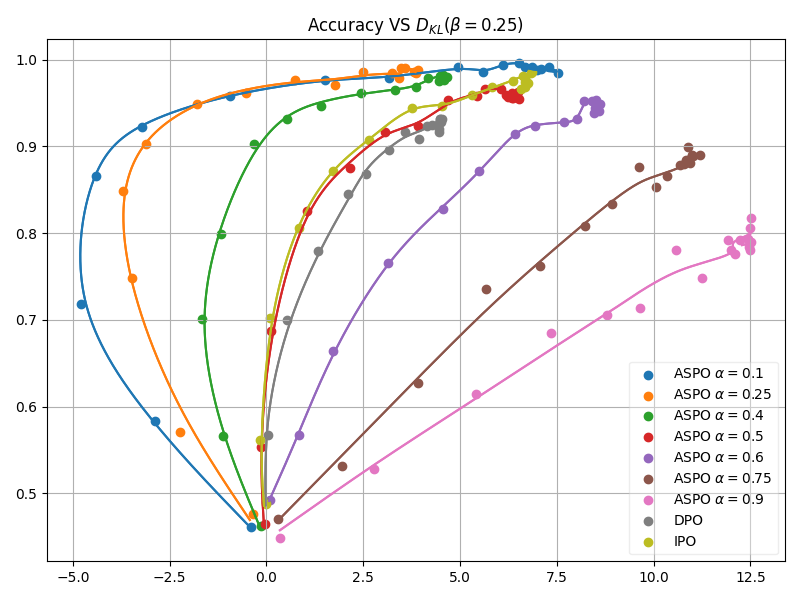
\includegraphics[width=0.85\textwidth]{./source/plots/1778263285_b0.25-filtered_acc_v_kl.png}
  \end{center}\caption{Зависимость точности от KL-дивергенции при $\beta=0.25$.}\label{fig:b025_1}
\end{figure}

\noindent\begin{figure}[H]
  \begin{center}
    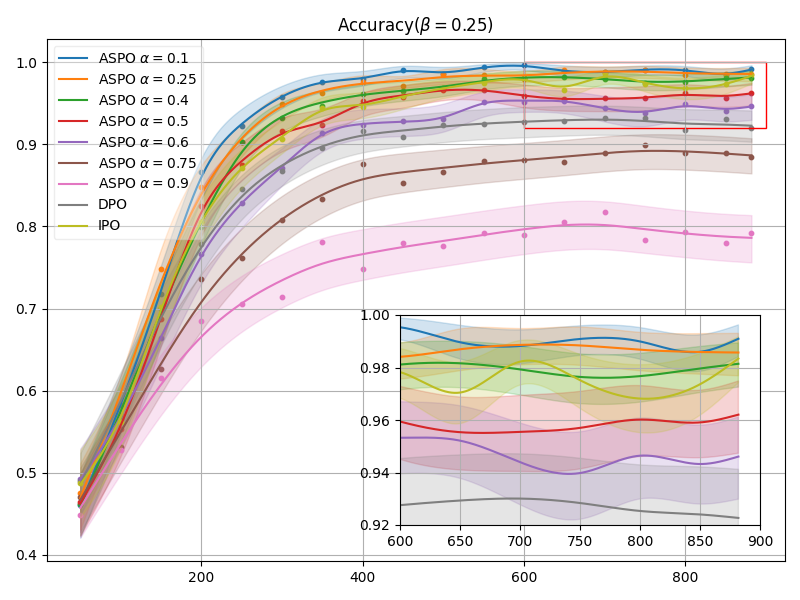
\includegraphics[width=0.85\textwidth]{./source/plots/1778263285_b0.25-filtered_acc_v_steps.png}
  \end{center}\caption{Зависимость точности от количества шагов обучения при $\beta=0.25$.}\label{fig:b025_2}
\end{figure}

\noindent\begin{figure}[H]
  \begin{center}
    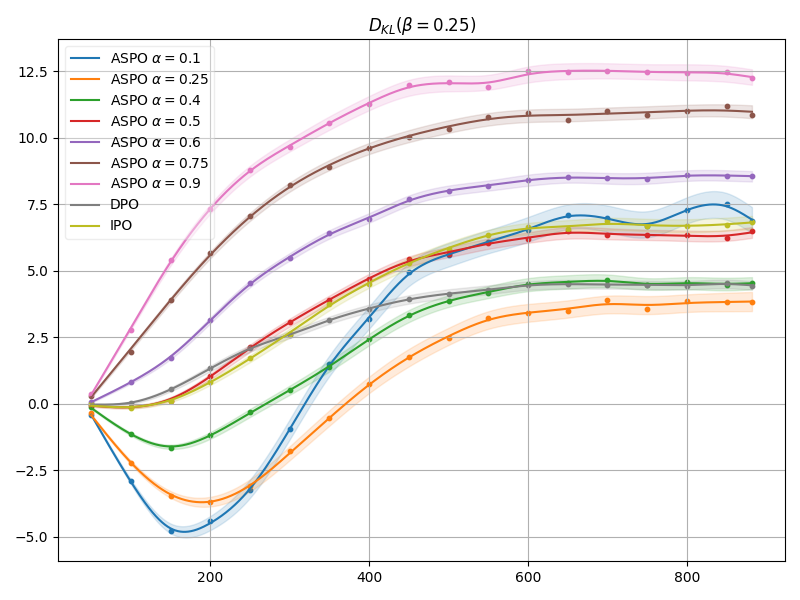
\includegraphics[width=0.85\textwidth]{./source/plots/1778263285_b0.25-filtered_kl_v_steps.png}
  \end{center}\caption{Зависимость KL-дивергенции от количества шагов обучения при $\beta=0.25$.}\label{fig:b025_3}
\end{figure}

\noindent\begin{figure}[H]
  \begin{center}
    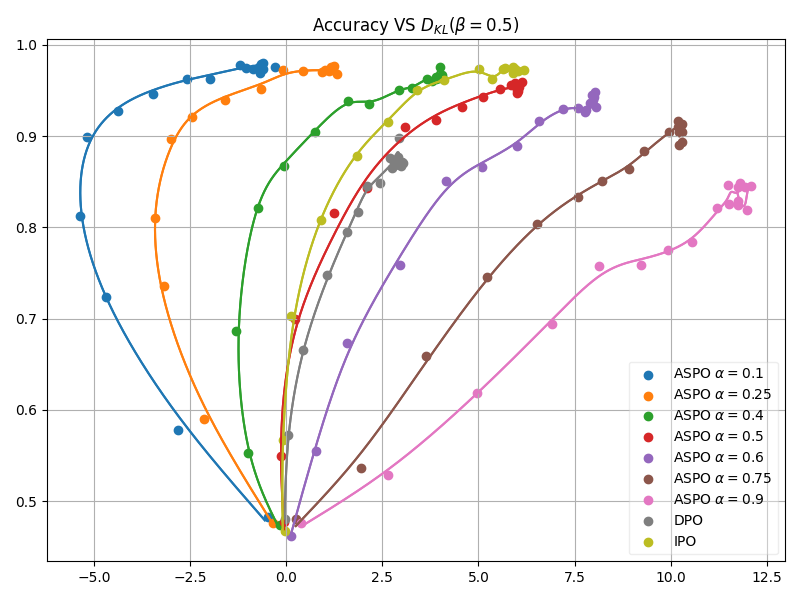
\includegraphics[width=0.85\textwidth]{./source/plots/1778226360_b0.5-filtered_acc_v_kl.png}
  \end{center}\caption{Зависимость точности от KL-дивергенции.}\label{fig:b05_1}
\end{figure}

\noindent\begin{figure}[H]
  \begin{center}
    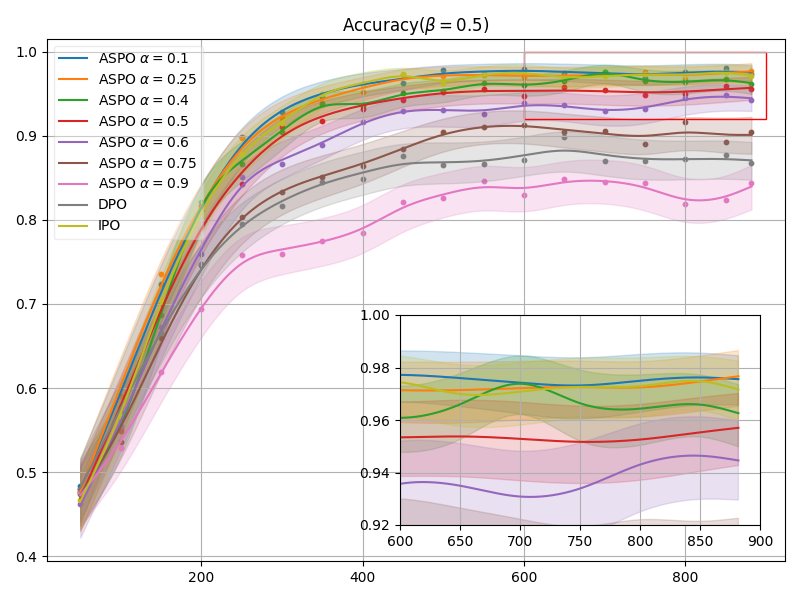
\includegraphics[width=0.85\textwidth]{./source/plots/1778226360_b0.5-filtered_acc_v_steps.png}
  \end{center}\caption{Зависимость точности от количества шагов обучения при $\beta=0.5$.}\label{fig:b05_2}
\end{figure}

\noindent\begin{figure}[H]
  \begin{center}
    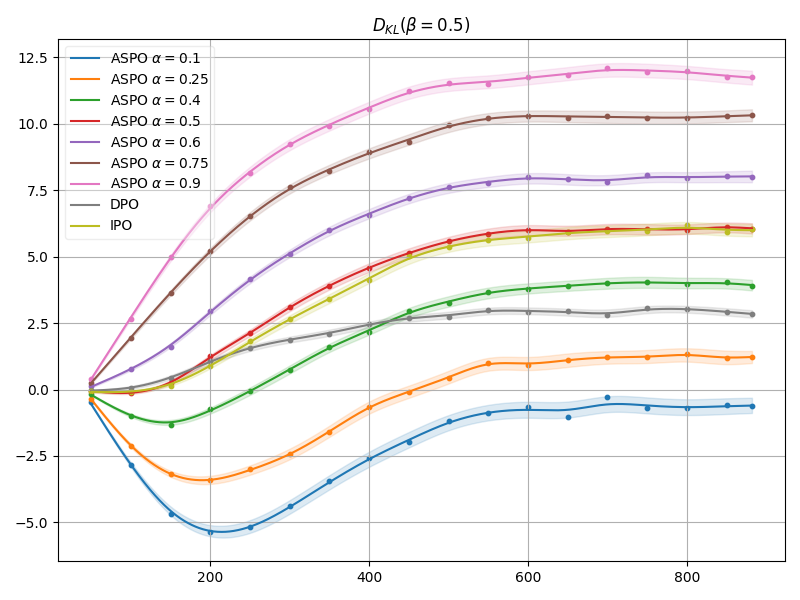
\includegraphics[width=0.85\textwidth]{./source/plots/1778226360_b0.5-filtered_kl_v_steps.png}
  \end{center}\caption{Зависимость KL-дивергенции от количества шагов обучения при $\beta=0.5$.}\label{fig:b05_3}
\end{figure}


\noindent\begin{figure}[H]
  \begin{center}
    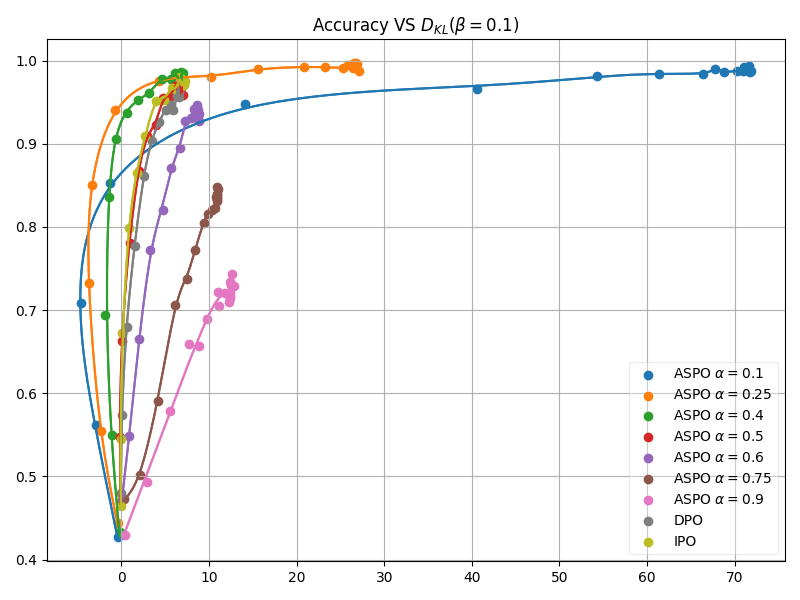
\includegraphics[width=0.85\textwidth]{./source/plots/1778214986_b0.1-filtered_acc_v_kl.png}
  \end{center}\caption{Зависимость точности от KL-дивергенции при $\beta=0.1$.}\label{fig:b01_1}
\end{figure}

\noindent\begin{figure}[H]
  \begin{center}
    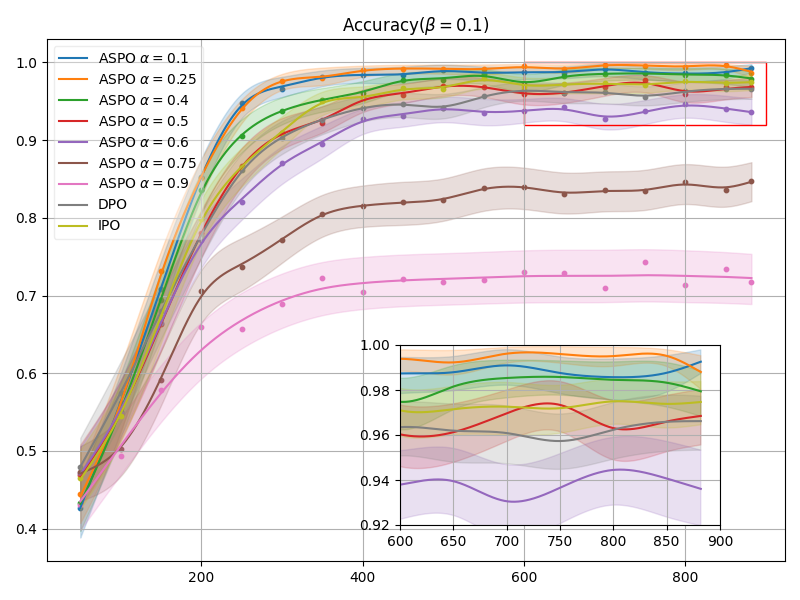
\includegraphics[width=0.85\textwidth]{./source/plots/1778214986_b0.1-filtered_acc_v_steps.png}
  \end{center}\caption{Зависимость точности от количества шагов обучения при $\beta=0.1$.}\label{fig:b01_2}
\end{figure}

\noindent\begin{figure}[H]
  \begin{center}
    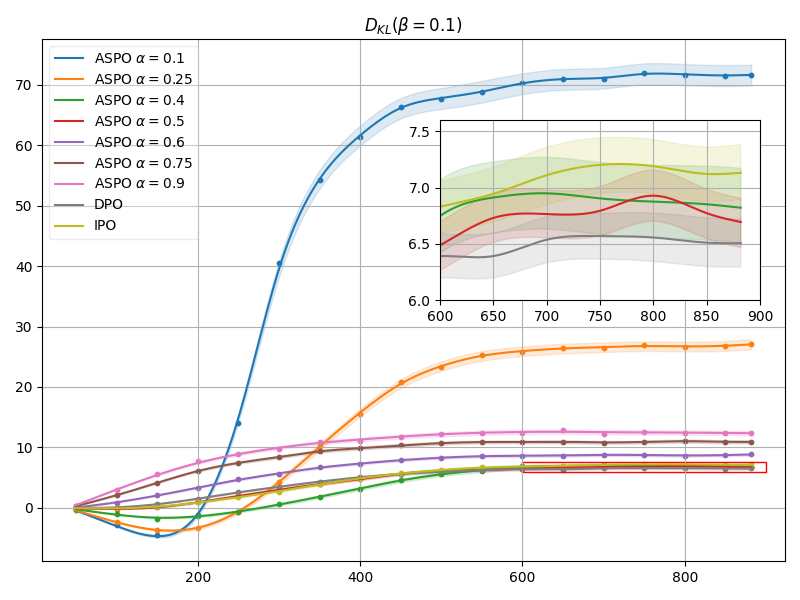
\includegraphics[width=0.85\textwidth]{./source/plots/1778214986_b0.1-filtered_kl_v_steps.png}
  \end{center}\caption{Зависимость KL-дивергенции от количества шагов обучения при $\beta=0.1$.}\label{fig:b01_3}
\end{figure}

\noindent\begin{enumerate}
    \item \textbf{Совпадение с IPO при $\alpha = 0.5$.} Для всех рассмотренных значений $\beta$ кривая ASPO с $\alpha = 0.5$ практически совпадает с кривой IPO.
    
    \item \textbf{Преимущество при $\alpha < 0.5$.} Уменьшение параметра $\alpha$ приводит к смещению кривой в область меньших значений KL при сохранении или даже незначительном повышении точности. Данный эффект объясняется свойством центрирования отступа. При $\alpha < 0.5$ центр отступа $\bar{r} = (2\alpha - 1)/(4\beta)$ смещается в отрицательную область. Такая асимметрия позволяет политике достигать требуемой разности $r_w - r_l = 1/(2\beta)$ с меньшим суммарным отклонением от исходной модели. При этом политика фокусируется не на усилении генерации выбранных ответов, а на предотвращении генерации отвергнутых. В результате при малых $\alpha$ распределение вероятностей на токенах, характерных для выбранных ответов, меняется незначительно по сравнению с исходной моделью, тогда как токены, типичные для отвергнутых ответов, активно подавляются.
    
    \item \textbf{Отрицательная KL-дивергенция.} При $\alpha < 0.25$  на ранних этапах обучения оценка KL-дивергенции становится отрицательной. С формальной точки зрения, KL-дивергенция неотрицательна по определению, однако её Монте-Карло оценка по токенам ответов, сгенерированных политикой, может принимать отрицательные значения — например, если для генерируемых последовательностей политика систематически назначает более низкие вероятности сэмплируемым токенам, чем исходная модель.
    
    \item \textbf{Зависимость оптимального $\alpha$ от $\beta$.} С увеличением $\beta$ оптимальное значение $\alpha$, при котором достигается наилучший компромисс точность–дивергенция, смещается ближе к $0.25$. При $\beta = 0.1$ наилучшие результаты достигаются при $\alpha \approx 0.4$, при $\beta = 0.5$ — при $\alpha \approx 0.25$.
\end{enumerate}






% =============================================
\section{Заключение}

В первой части работы была выстроена общая теоретическая основа, объединяющая ключевые принципы прямой оптимизации предпочтений. Для этого введена единая система обозначений. На этой базе показано, как современные методы (DPO, IPO) осуществляют выравнивание языковых моделей непосредственно на парах предпочтений, исключая стадию обучения модели вознаграждения. В работе представлены математические обоснования выбора функций потерь, сформулированы условия оптимальности. На основе сравнения подходов разработан экспериментальный алгоритм ASPO — модификация IPO с раздельной регуляризацией, обеспечивающая центрирование отступа между оценками ответов и управляемую асимметрию обучения.

Во второй части работы представлена экспериментальная проверка рассмотренных алгоритмов. Экспериментальный анализ подтвердил, что ASPO сохраняет теоретические гарантии оптимальности IPO и предоставляет дополнительную гибкость за счёт параметра $\alpha$. При $\alpha < 0.5$ достигается улучшение компромисса «точность против KL-дивергенции», а при $\alpha = 0.5$ поведение алгоритма схоже с IPO.

% =============================================
% Библиография
% =============================================
\newpage
\begin{thebibliography}{99}

\bibitem{ouyang2022training}
Ouyang L., Wu J., Jiang X. et al. Training language models to follow instructions with human feedback // Advances in Neural Information Processing Systems (NeurIPS). -- 2022. -- Vol.~35. -- P.~27730--27744.

\bibitem{rafailov2023direct}
Rafailov R., Sharma A., Mitchell E. et al. Direct Preference Optimization: Your Language Model is Secretly a Reward Model // Advances in Neural Information Processing Systems (NeurIPS). -- 2023.

\bibitem{azar2024general}
Azar M.~G., Rowland M., Piot B. et al. A General Theoretical Paradigm to Understand Learning from Human Preferences // Proceedings of the 27th International Conference on Artificial Intelligence and Statistics (AISTATS). -- 2024. -- P.~4447--4455.

\bibitem{vonwerra2022trl}
von Werra L., Belkada Y., Tunstall L. et al. TRL: Transformer Reinforcement Learning [Электронный ресурс] // GitHub. -- 2022. -- Режим доступа: \texttt{https://github.com/huggingface/trl}.

\bibitem{kingma2014adam}
Kingma D.~P., Ba J. Adam: A Method for Stochastic Optimization // Proceedings of the 3rd International Conference on Learning Representations (ICLR). -- 2015.

\bibitem{liquidAI2026350M}
Liquid AI. LFM2.5-350M: No Size Left Behind // Liquid AI Blog. -- 2026. -- Режим доступа: \texttt{www.liquid.ai/blog/lfm2-5-350m-no-size-left-behind}.

\bibitem{hartmann2023}
Hartmann J., Heitmann M., Siebert C., Schamp C. More than a Feeling: Accuracy and Application of Sentiment Analysis // International Journal of Research in Marketing. -- 2023. -- Vol.~40, №~1. -- P.~75--87.

\bibitem{maas2011learning}
Maas A.~L., Daly R.~E., Pham P.~T., Huang D., Ng A.~Y., Potts C. Learning Word Vectors for Sentiment Analysis // Proceedings of the 49th Annual Meeting of the Association for Computational Linguistics: Human Language Technologies (ACL-HLT). -- Portland, Oregon, USA, 2011. -- P.~142--150.

\end{thebibliography}


\end{document}